\section{Experiment Results}
\label{sec:experiments:results}

In this section, we present the results obtained from the experiments as defined in \cref{sec:experiments:design:overview}. We first present the main findings in \cref{sec:experiments:main-findings}. After this, we present and explain how to interpret the results per experiment in \cref{sec:experiments:results:per-experiment} and discuss these findings in greater detail.

\subsection{Main Findings}
\label{sec:experiments:main-findings}
% Significant decrease in throughput
% Additional avg latency, esp tail ends. p99+
% Traefik experiences bottlenecks, bimodal distribution
% Istio consumes most CPU resources
% Applications Payloads seem to have little effect on performance
% Application protocol seems to have little impact, although linkerd performs a bit worse on gRPC throughput
% Traefik failed to handle gRPC worklaods
% Cilium best allround performer

We now present the main findings of the conducted experiments.

\begin{enumerate}[label=\textbf{MF\arabic*}, leftmargin=3\parindent]
    \item \textbf{There can be a significant drop in maximum throughput when using a service mesh}
    \label{exp:mf1}
    Every service mesh suffers from a decrease in maximum throughput. The observed decrease in throughput varies greatly, with a best-case scenario having a  $-16.8\%$ decrease while the worst performing configuration has a significant  $-97.38\%$ decrease in maximum throughput.
    
    \item \textbf{There can be a significant increase in request latencies when using a service mesh}
    \label{exp:mf2}
    A service mesh introduces additional request latency by introducing a network proxy in front of the service. This additional overhead, however, can have a large impact on average and tail end request latencies as observed. With the best performing mesh increasing the average request latency with $20.27\%$ whereas the worst performing configuration saw a staggering $3720.95\%$ uplift.
    
    \item \textbf{Traefik mesh experiences bottlenecks after it reaches a certain throughput threshold}
    \label{exp:mf3}
    We observed that \textit{Traefik} cannot perform above a certain throughput level, and will throttle requests, resulting in a bimodal distribution of request latencies and a significant loss of performance for those requests.
    
    \item \textbf{Istio is the most demanding in terms of CPU utilization}
    \label{exp:mf4}
    We observe that \textit{Istio} consumes significantly more CPU resources compared to other configurations. We also observe that this is due to its data plane proxy which does not scale as well as the proxies in other configurations.
    
    \item \textbf{Application payloads have little to no effect on the observed performance}
    \label{exp:mf5}
    We observed that increasing the application payload, has little to no effect on the performance of meshed configurations.
    
    \item \textbf{Application level protocols have little to no effect on the observed performance}
    \label{exp:mf6}
    We observed that different layer 7 protocols, HTTP vs gRPC, had little to no impact on the decrease in throughput observed.
    
    \item \textbf{Traefik was unable to handle gRPC workloads}
    \label{exp:mf7}
    We observed that \textit{Traefik} was unable to handle and execute gRPC workloads in our experiments even though it listed explicit support for gRPC.
    
    \item \textbf{Cilium was the best all-round performing configuration, with a significant margin}
    \label{exp:mf8}
    We observed that the configuration using \textit{Cilium} outperformed any other configuration using a \gls{sm} with significant margins in all the experiments that were conducted.
\end{enumerate}



\subsection{Results per Experiment}
\label{sec:experiments:results:per-experiment}

We now present the results of each individual experiment and discuss how to interpret them.

\subsubsection{\ref{exp:design:1} - HTTP Maximum Throughput}
\label{sec:experiments:results:per-experiment:01}
% Goal:
% To find the maximum throughput each of the meshed configurations can achieve.

% Introduce all figures
The goal of the first experiment was to determine the maximum throughput of each meshed configuration. The results of this experiment are depicted in \cref{fig:exp:result:01:latency}, \cref{fig:exp:result:01:cpu} and \cref{fig:exp:result:01:memory}. 

% Histogram results
% How to read results
The first illustration (\cref{fig:exp:result:01:latency}), depicts a histogram that shows the distribution of request latencies for each meshed configuration. The x-axis represents the latency expressed in milliseconds in a logarithmic fashion. The left y-axis is related to the bars in the histogram and represents the number of requests. The right y-axis is related to the cumulative density function line (the yellow line on top of the histogram) and represents the proportion of requests. Each bar represents a bin of the histogram, and all bins in the histogram can be of varying sizes. The bins closer to the expected latency are smaller, whereas bins further away from the expected latency can cover larger areas. Additionally, each plot in the figure is accompanied by descriptive statistics such as the minimum, average and maximum request duration. Furthermore, it also contains the achieved throughput, expressed as requests per second (\textbf{RPS}).


\begin{figure}[!t]
    \centering
    
    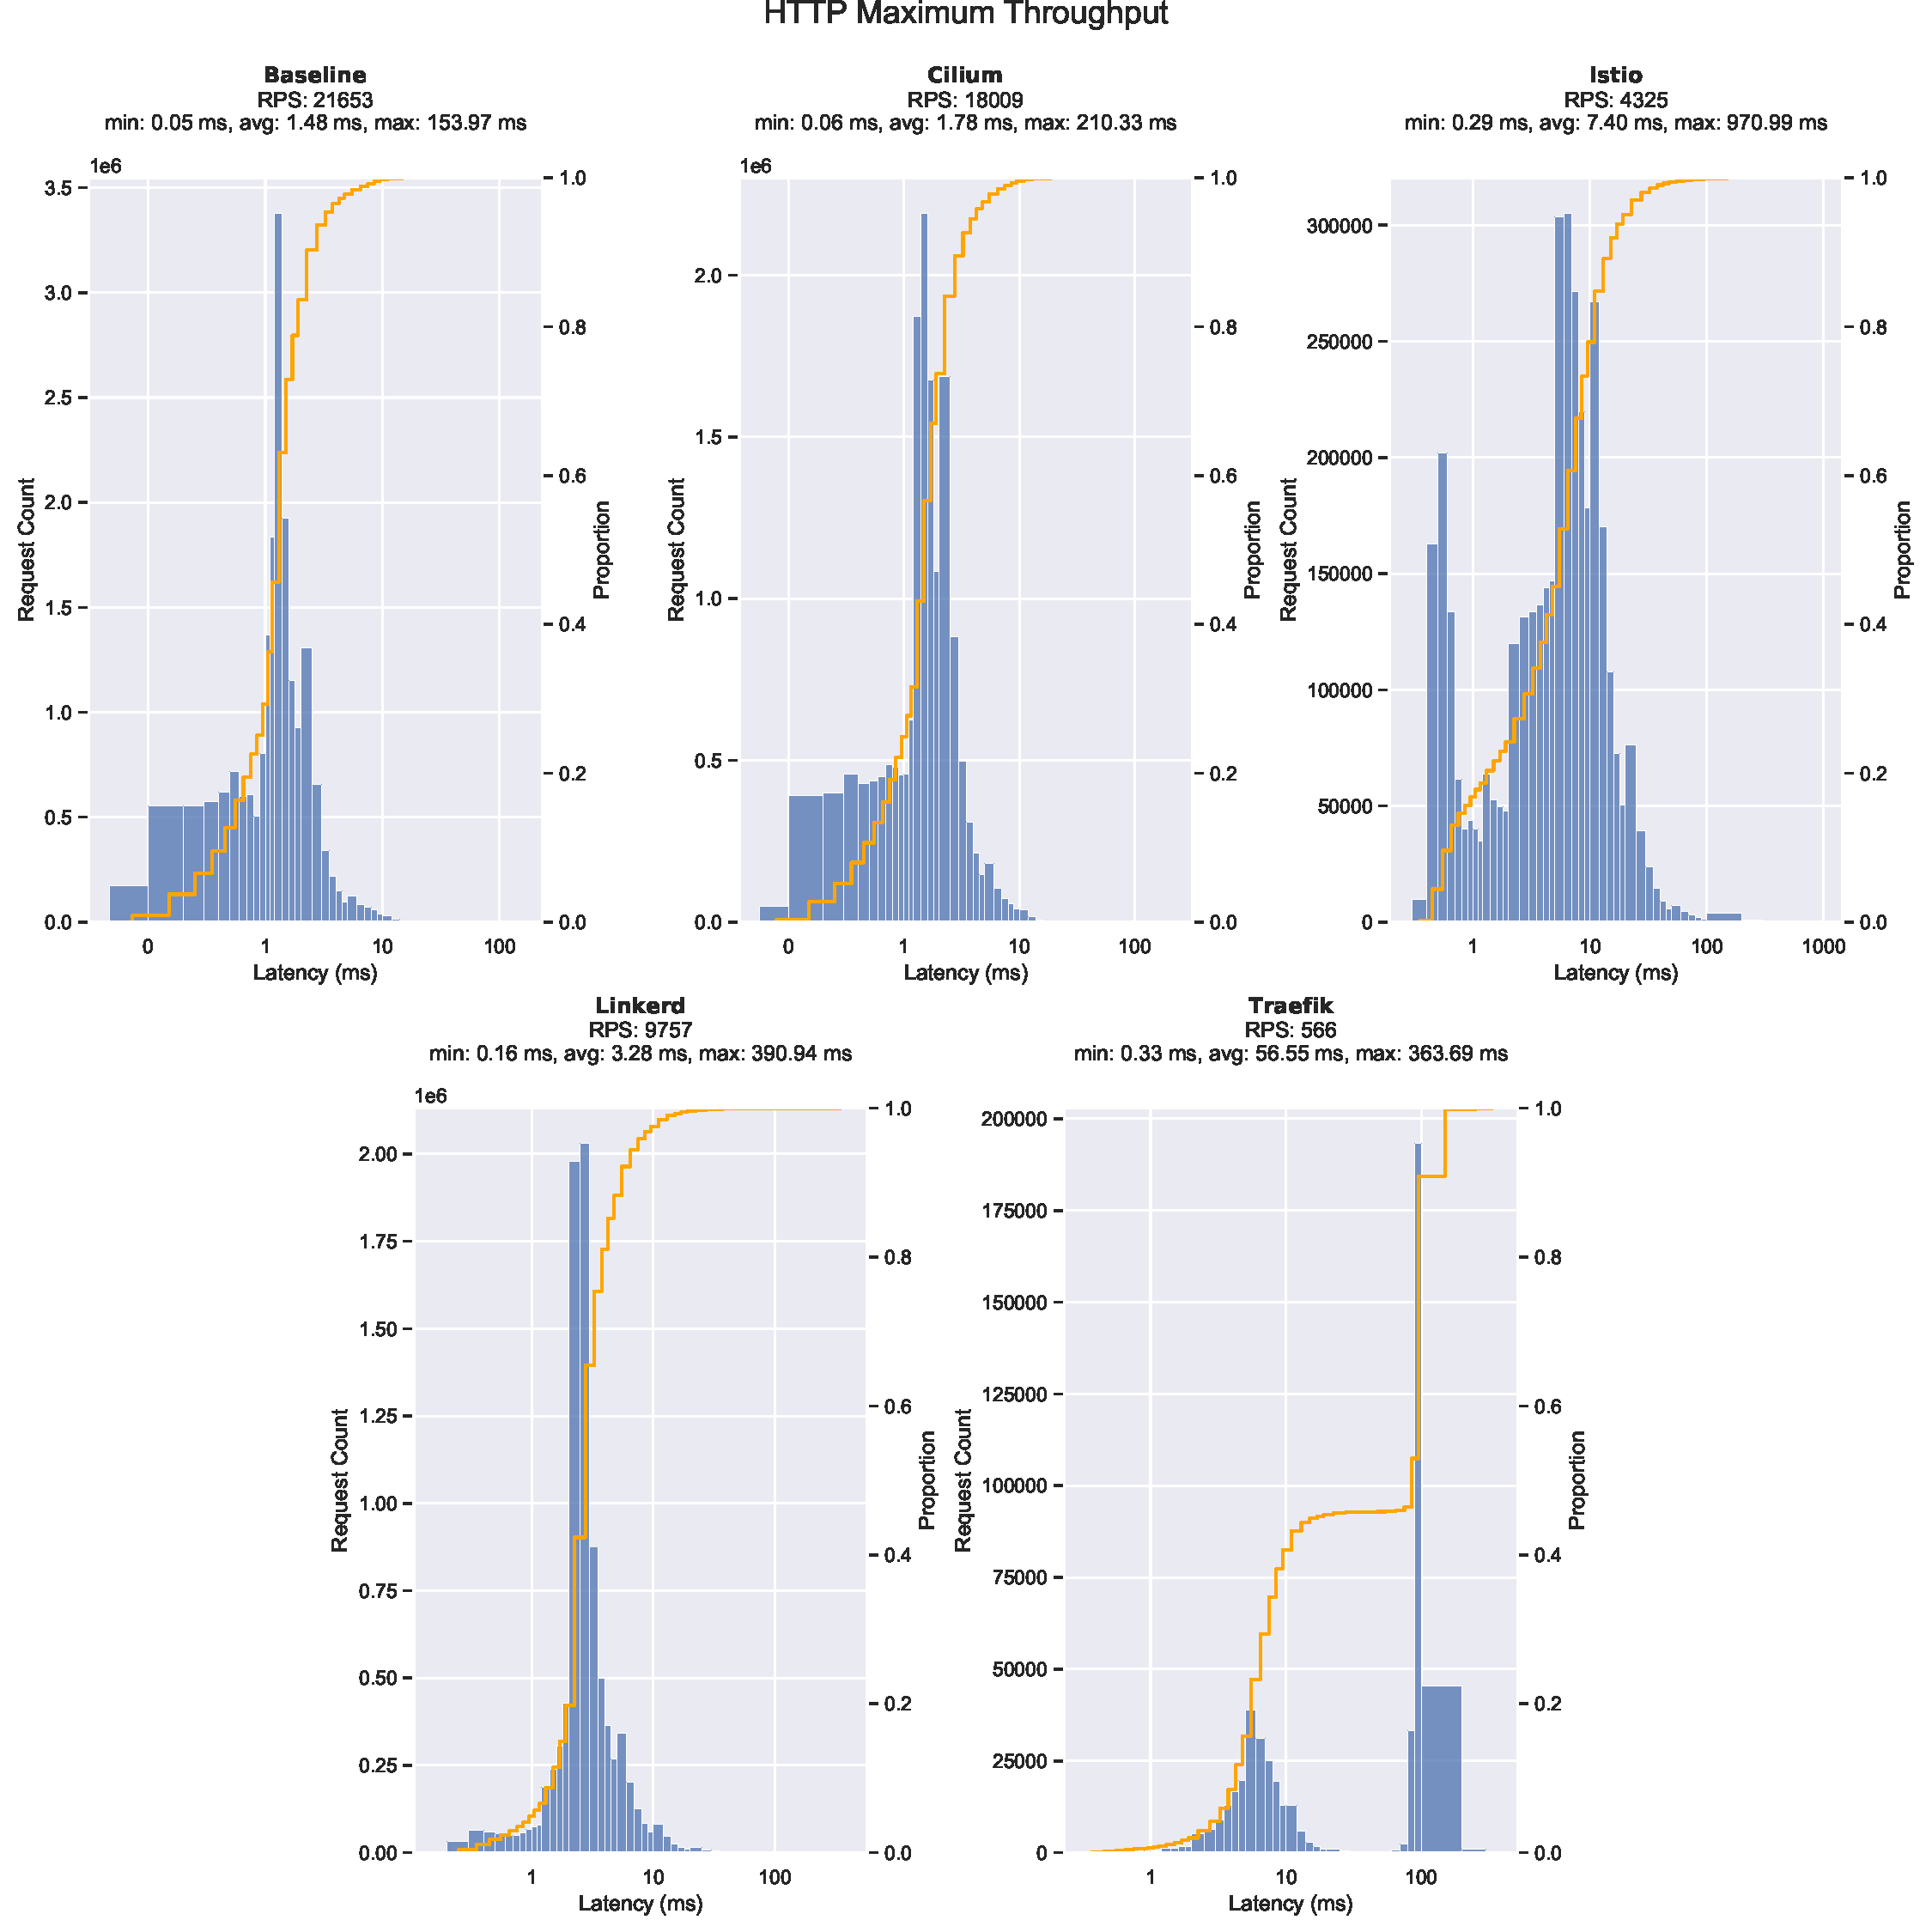
\includegraphics[width=\linewidth]{5_experimental_evaluation/figures/exp_01-latency-results.pdf}

    \caption{\ref{exp:design:1} - Latency Results}
    
    \label{fig:exp:result:01:latency}
\end{figure}



% Findings
% - Baseline best (highest RPS, best latency avg)
% - Distributions roughly normal
% - Large increases in average/tail end latencies
% - Traefik mesh bimodal distribution
% cilium QPS diff: -16.827679769486704%
% istio QPS diff: -80.0264142981776%
% linkerd QPS diff: -54.940993873502805%
% traefik QPS diff: -97.38692130213765%
From the histograms in \cref{fig:exp:result:01:latency} we can observe that the baseline performs the best, i.e. it has the highest observed throughput and the minimum, average and maximum latencies outperform any meshed configuration. In terms of achieved throughput, \textit{Cilium} performs second best and loses $-16.83\%$ compared to the baseline configuration with no \gls{sm} applied. The configuration using \textit{Linkerd}, however, lost more than half ($-54.94\%$), whereas the situation for \textit{Istio} and \textit{Traefik} was even worse as they saw a throughput drop of $-80.26\%$ and $-97.39\%$ respectively. Another interesting observation can be made when looking at the average latencies and tail end latencies for the meshed configurations compared to the baseline measurements. First, we can see a minor increase in average latency for \textit{Cilium}. More interestingly, however, we can see a $+121.62\%$ increase for the \textit{Linkerd} configuration compared to the baseline. The results for the \textit{Istio} configuration is even worse, where it sees an uplift of $+400\%$ for the average request latency compared to the baseline. \textit{Traefik}, however, sees the largest increase with a massive $+3720.95\%$ uplift in average request latency. When taking a closer look at the distributions in the histograms we can also notice that the configuration using the \textit{Traefik} mesh has a bimodal distribution, where one mode is around 8 milliseconds and another mode exists around the 100 millisecond mark.

% Explanation CPU/Mem line plots
In \cref{fig:exp:result:01:cpu} and \cref{fig:exp:result:01:memory} we depict the CPU and memory utilization results of the experiment. Both illustrations come in the form of line plots that have their metric expressed on the y-axis, for the CPU usage this is represented as fractions of a CPU core for both user and kernel time and for the memory utilization this is expressed in kilobytes used. On the x-axis we depict the time delta of the experiment since the start in minutes, each experiment takes 15 minutes and the lines in the plot show the resource utilization values over time. Additionally, each plot can have multiple lines, with one line for each container relevant to the configuration. In other words, we track the resource utilization for the containers related to the data path of the network traffic. In the baseline configuration this is only one experiment, since it does not employ a \gls{sm}, but in the meshed configurations proxy containers are plotted as well as indicated by the legends above the figures.

\begin{figure}[!t]
    \centering
    
    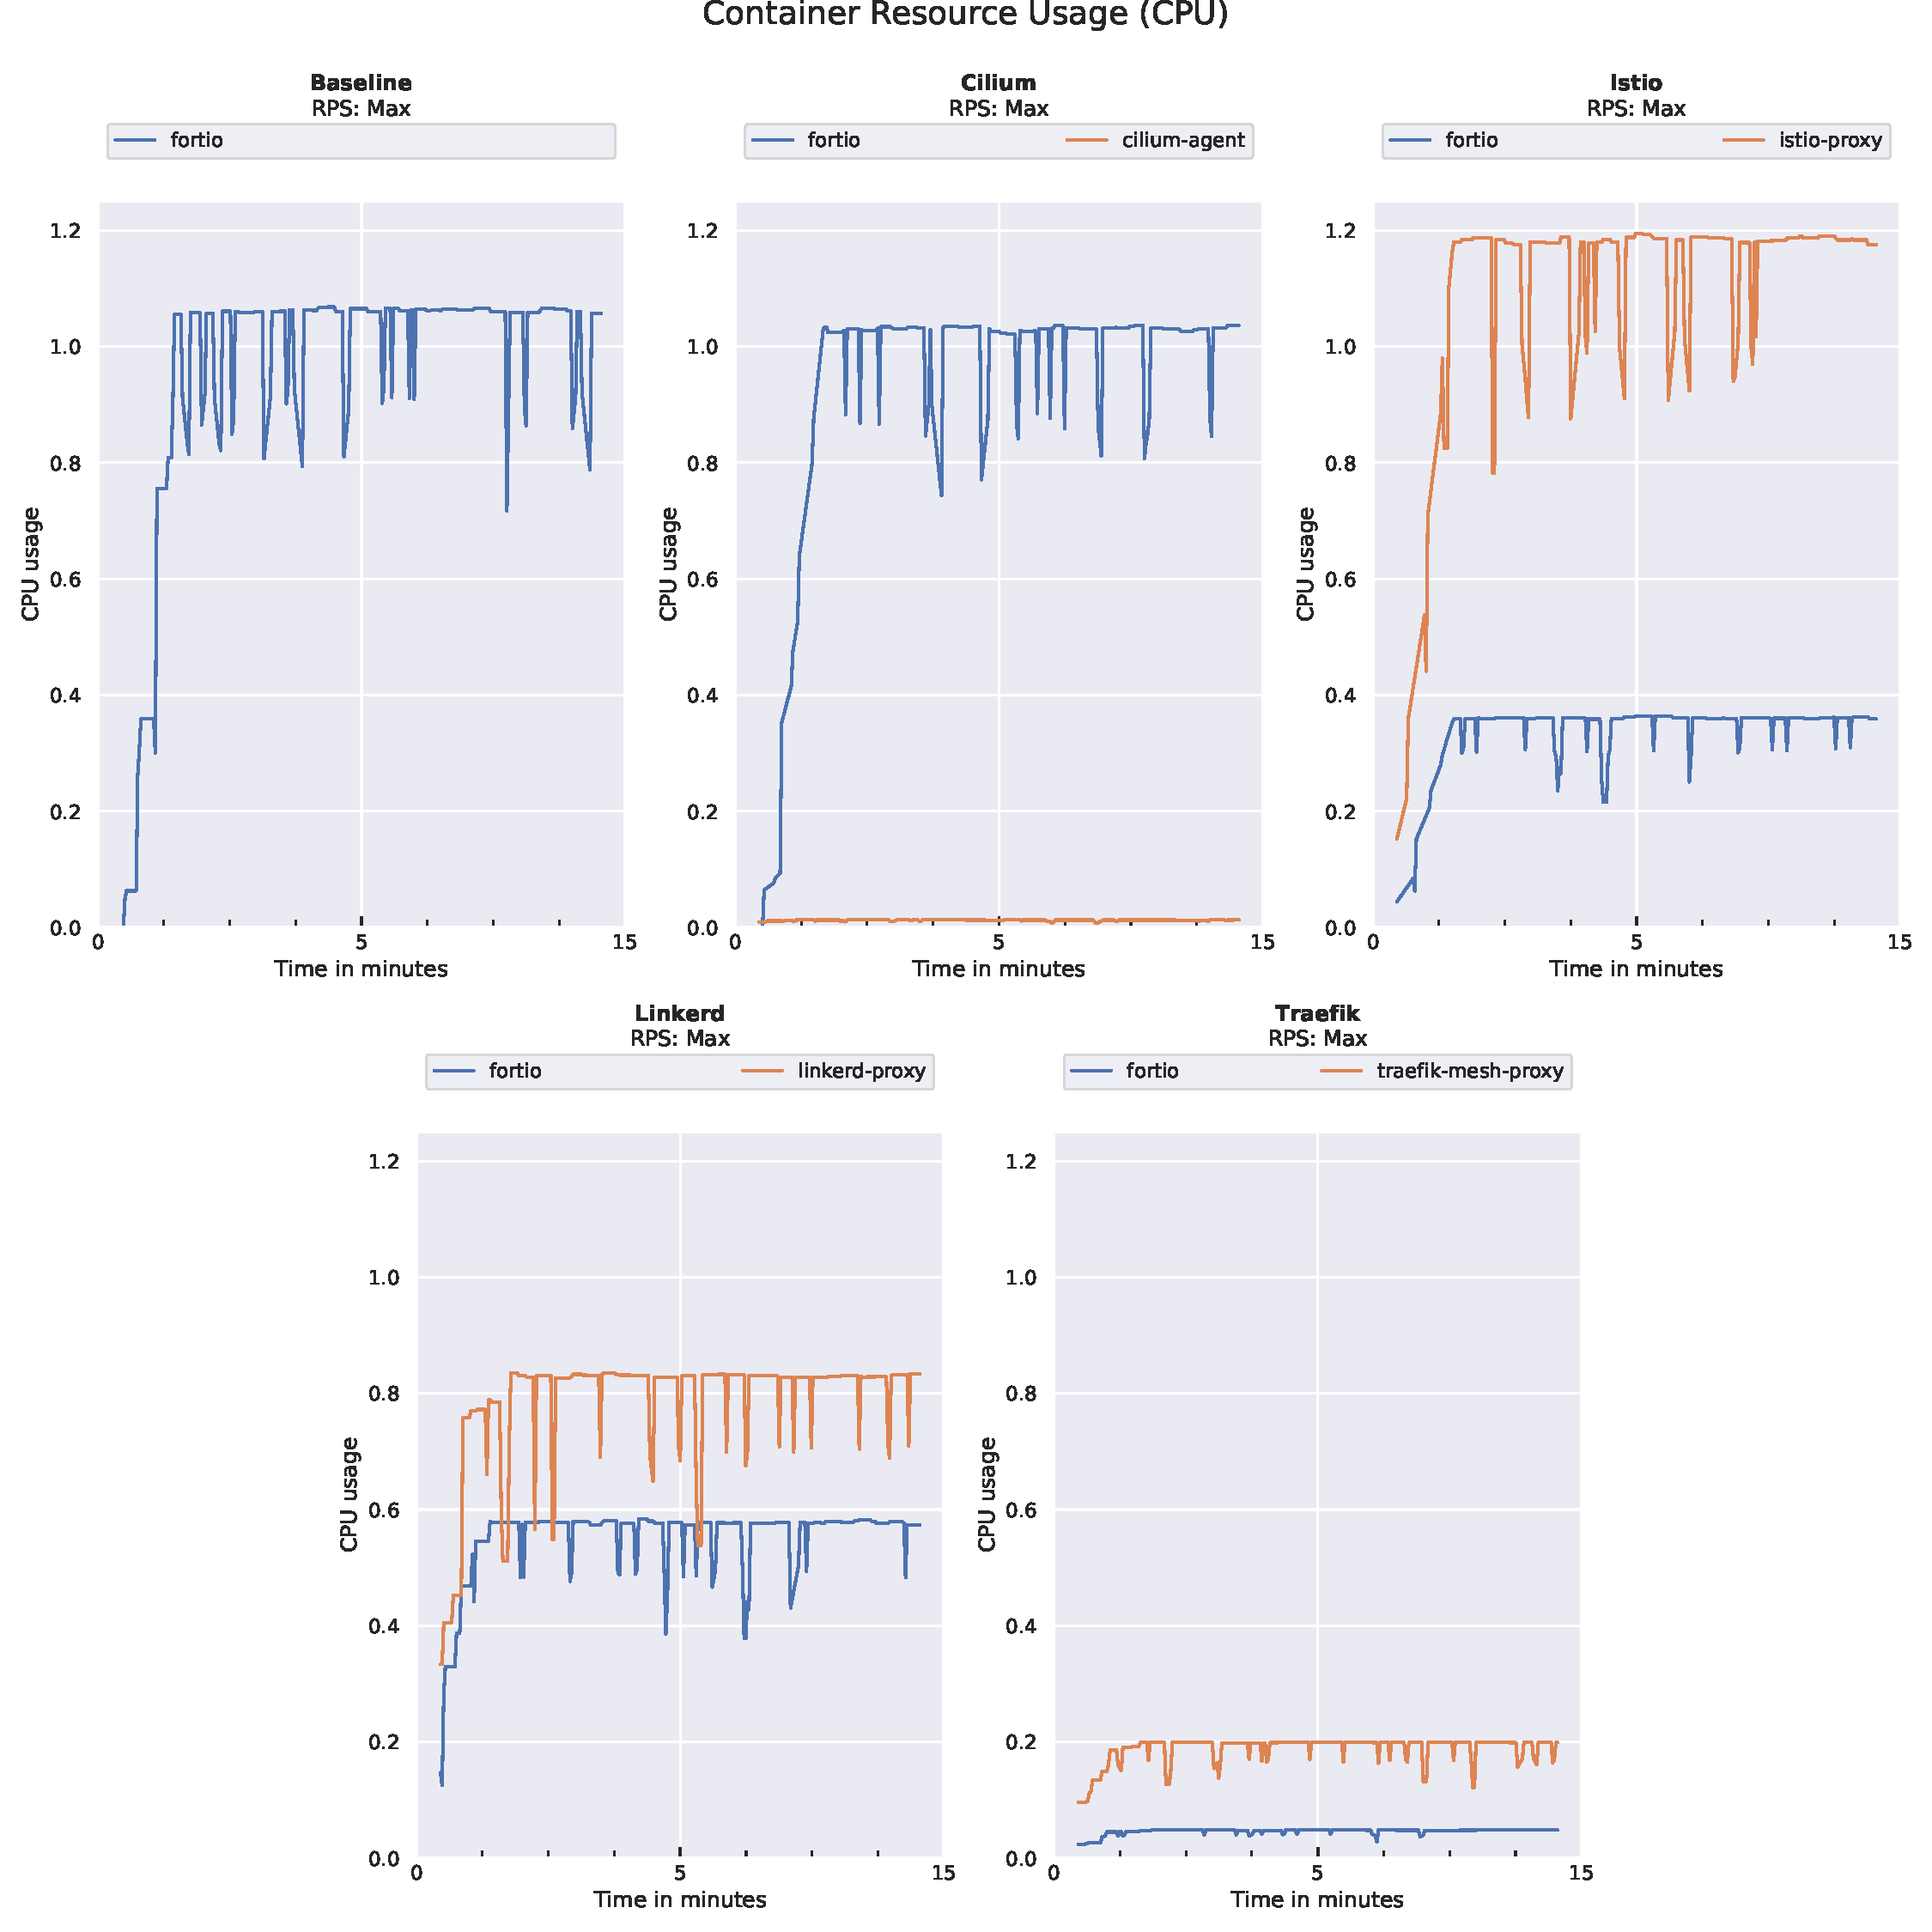
\includegraphics[width=\linewidth]{5_experimental_evaluation/figures/exp_01-cpu-results.pdf}

    \caption{\ref{exp:design:1} - CPU utilization results.}
    
    \label{fig:exp:result:01:cpu}
\end{figure}


% Notable findings
% Small rampup time
% 'fortio' usage -> RPS
% Istio-proxy high utilization
% Linkerd less, but more throughput
% Cilium very low utilization
% Traefik low -> bottleneck?
From the line plots in \cref{fig:exp:result:01:cpu} we can observe that for each configuration there is a small ramp-up time until the CPU utilization settles in. Furthermore, we can observe and relate back to our results depicted in the histograms (\cref{fig:exp:result:01:latency}) that there is a direct correlation between CPU utilization and throughput for the \textit{fortio} container (the target service that represents an echo server), as the meshed configurations that achieved less throughput have an inverse relation on CPU utilization. Interesting observations can be made regarding the CPU utilization of the service proxies. First of, \textit{Cilium}, with their kernel based proxying solution (\cref{{sec:survey:results:comparison:proxy}}) seems to have very little overhead compared to other proxying solutions. Second, the proxy used in the \textit{Istio} configuration appears to have the highest overhead, taking up more than an entire CPU core. Additionally, the proxy used in the \textit{Linkerd} configuration uses less CPU resources, which indicates that this solution is more efficient than \textit{Linkerd}'s proxy as it was able to handle a higher throughput as well. Finally, we observe that the \textit{Traefik} configuration used very CPU little resources at all, indicating bottlenecks of some sort.

From the plots depicting memory consumption in \cref{fig:exp:result:01:memory} we can see that for each configuration the memory usage was very minimal. The \textit{cilium-agent} container reached a spike and consumed at most $2.27$MB during maximum load. This amount is negligible for most systems and indicates that the data path proxies will likely not be memory constrained.

\begin{figure}[!t]
    \centering
    
    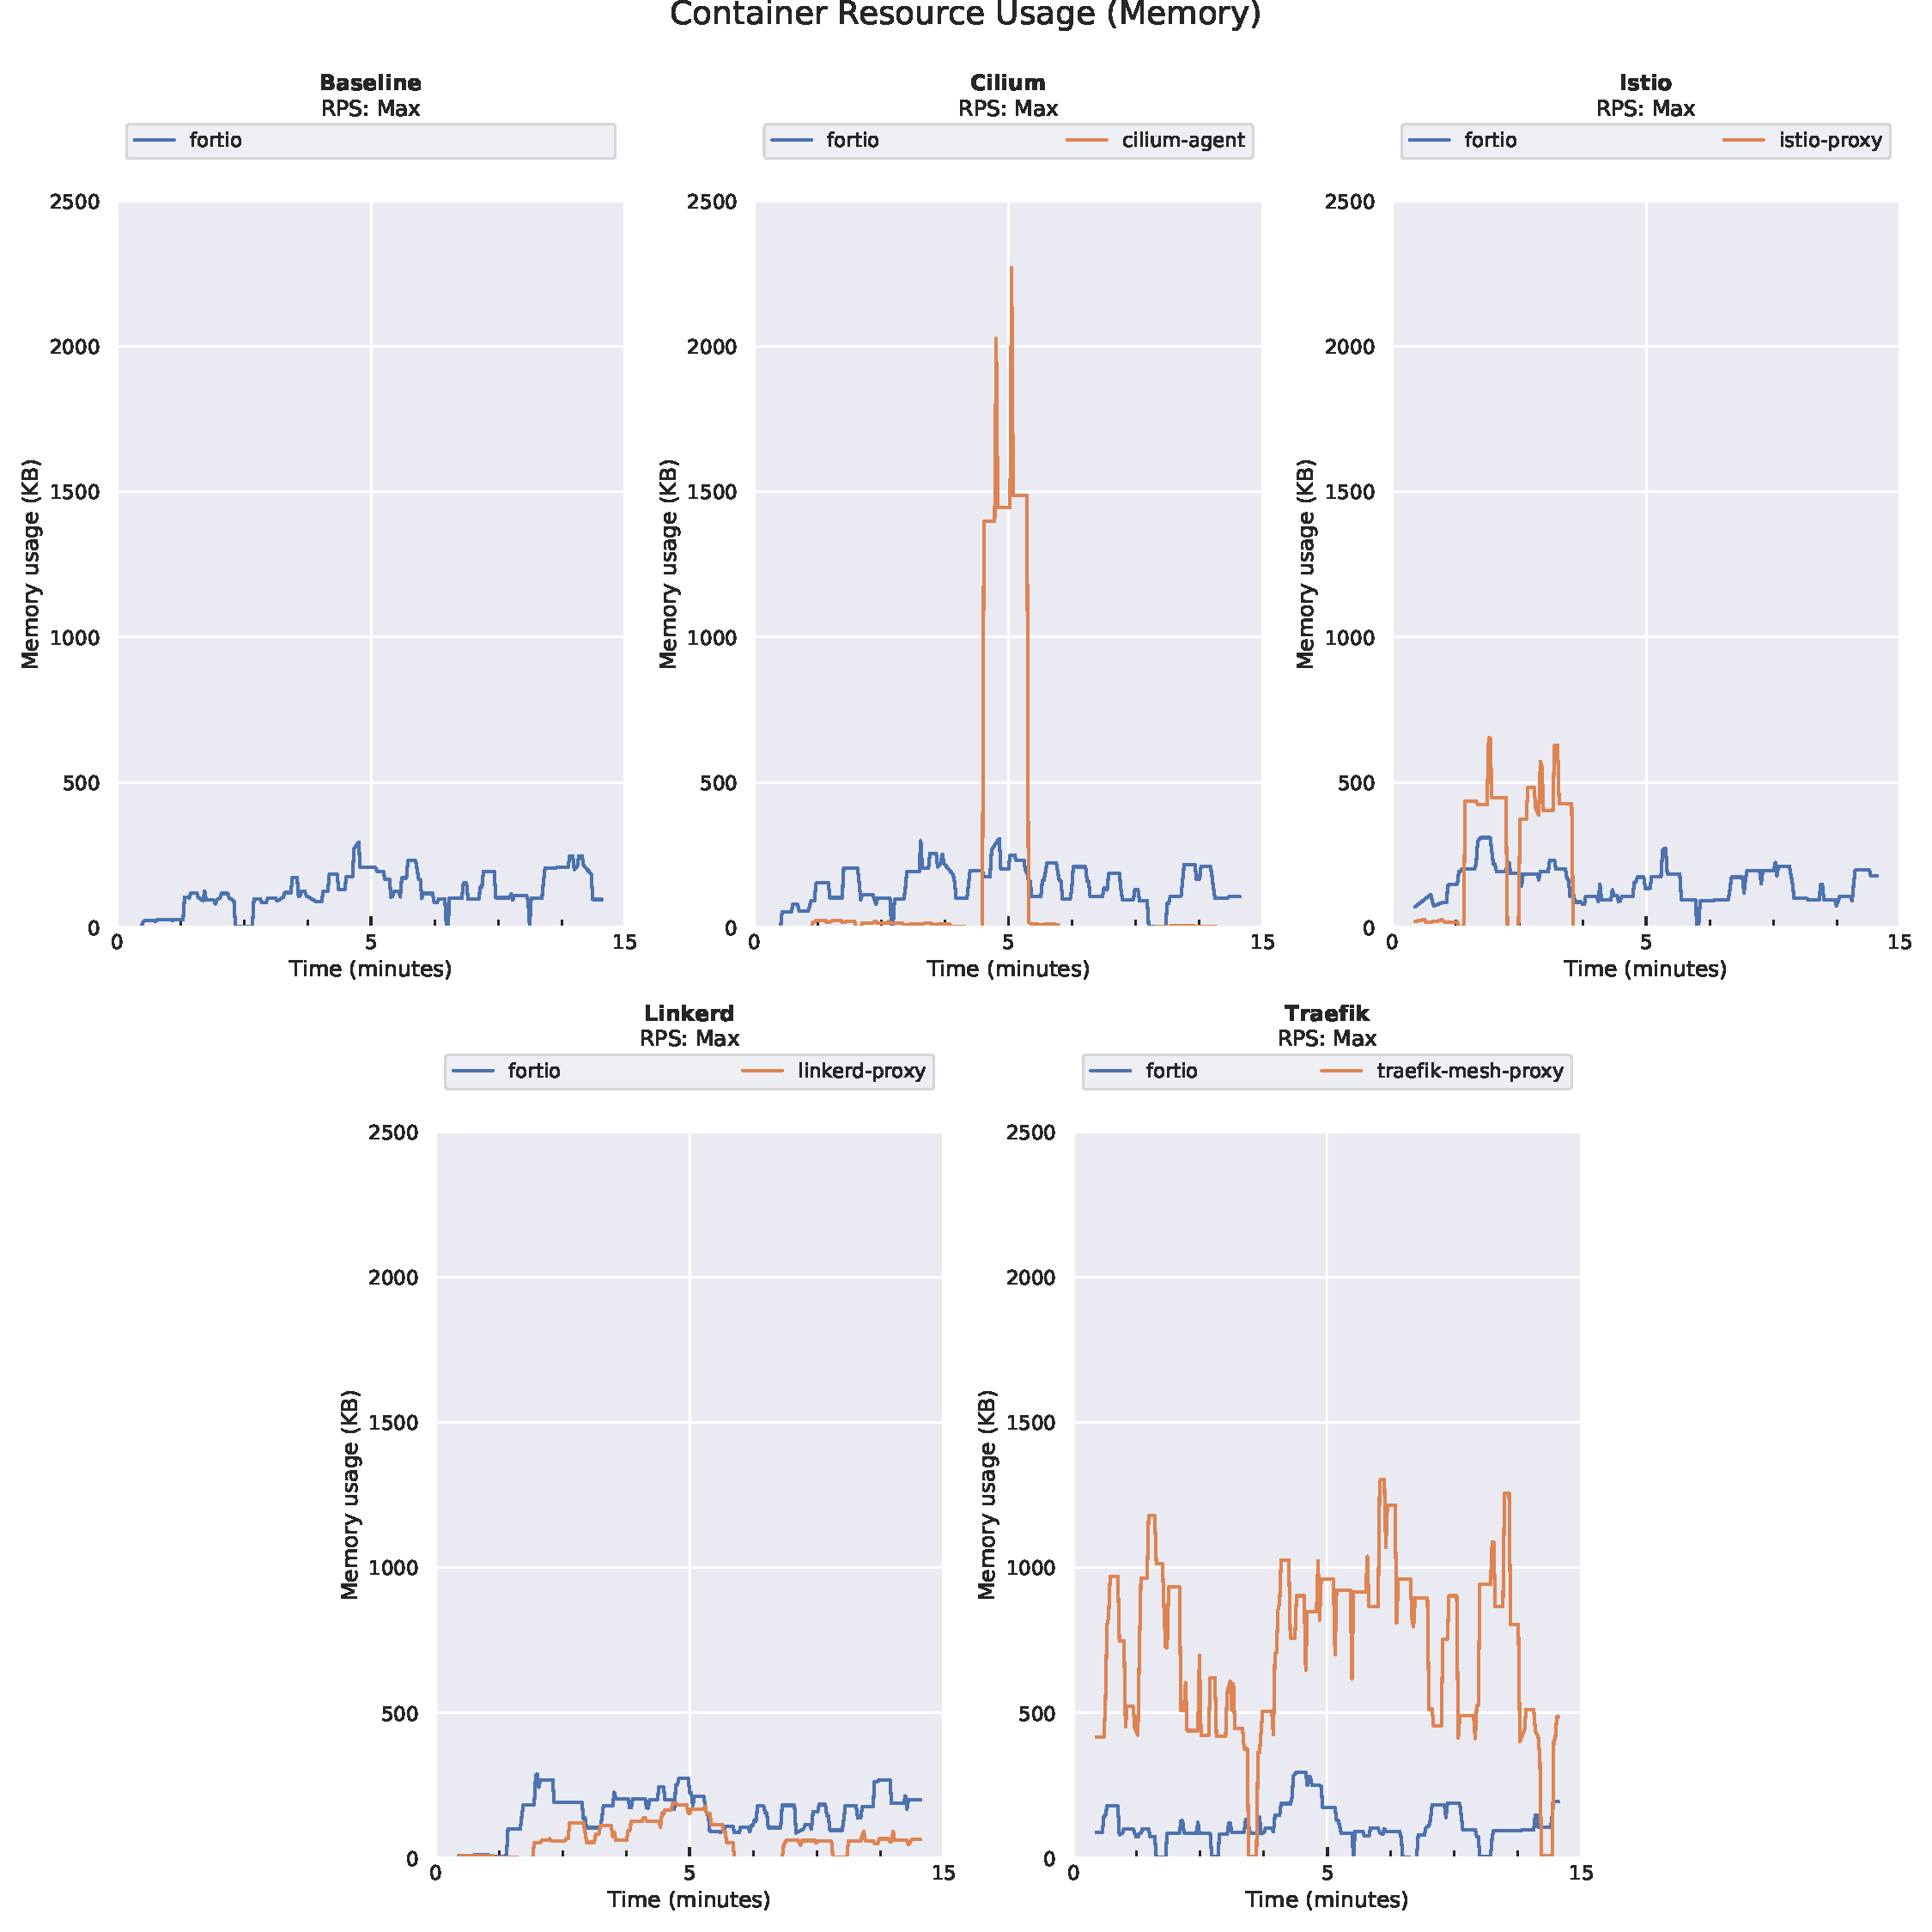
\includegraphics[width=\linewidth]{5_experimental_evaluation/figures/exp_01-memory-results.pdf}

    \caption{\ref{exp:design:1} - Memory Results}
    
    \label{fig:exp:result:01:memory}
\end{figure}



\subsubsection{\ref{exp:design:2} - HTTP Constant Throughput}
\label{sec:experiments:results:per-experiment:02}
% Goal: To evaluate how \gls{sm} configurations behave under varying levels of load.

The second experiment had as goal to evaluate the different \gls{sm} configurations under predefined levels of constant throughput. The results of this experiment are depicted in \cref{fig:exp:result:02:latency}, \cref{fig:exp:result:02:cpu} and \cref{fig:exp:result:02:memory}.


\begin{figure}[!t]
    \centering
    
    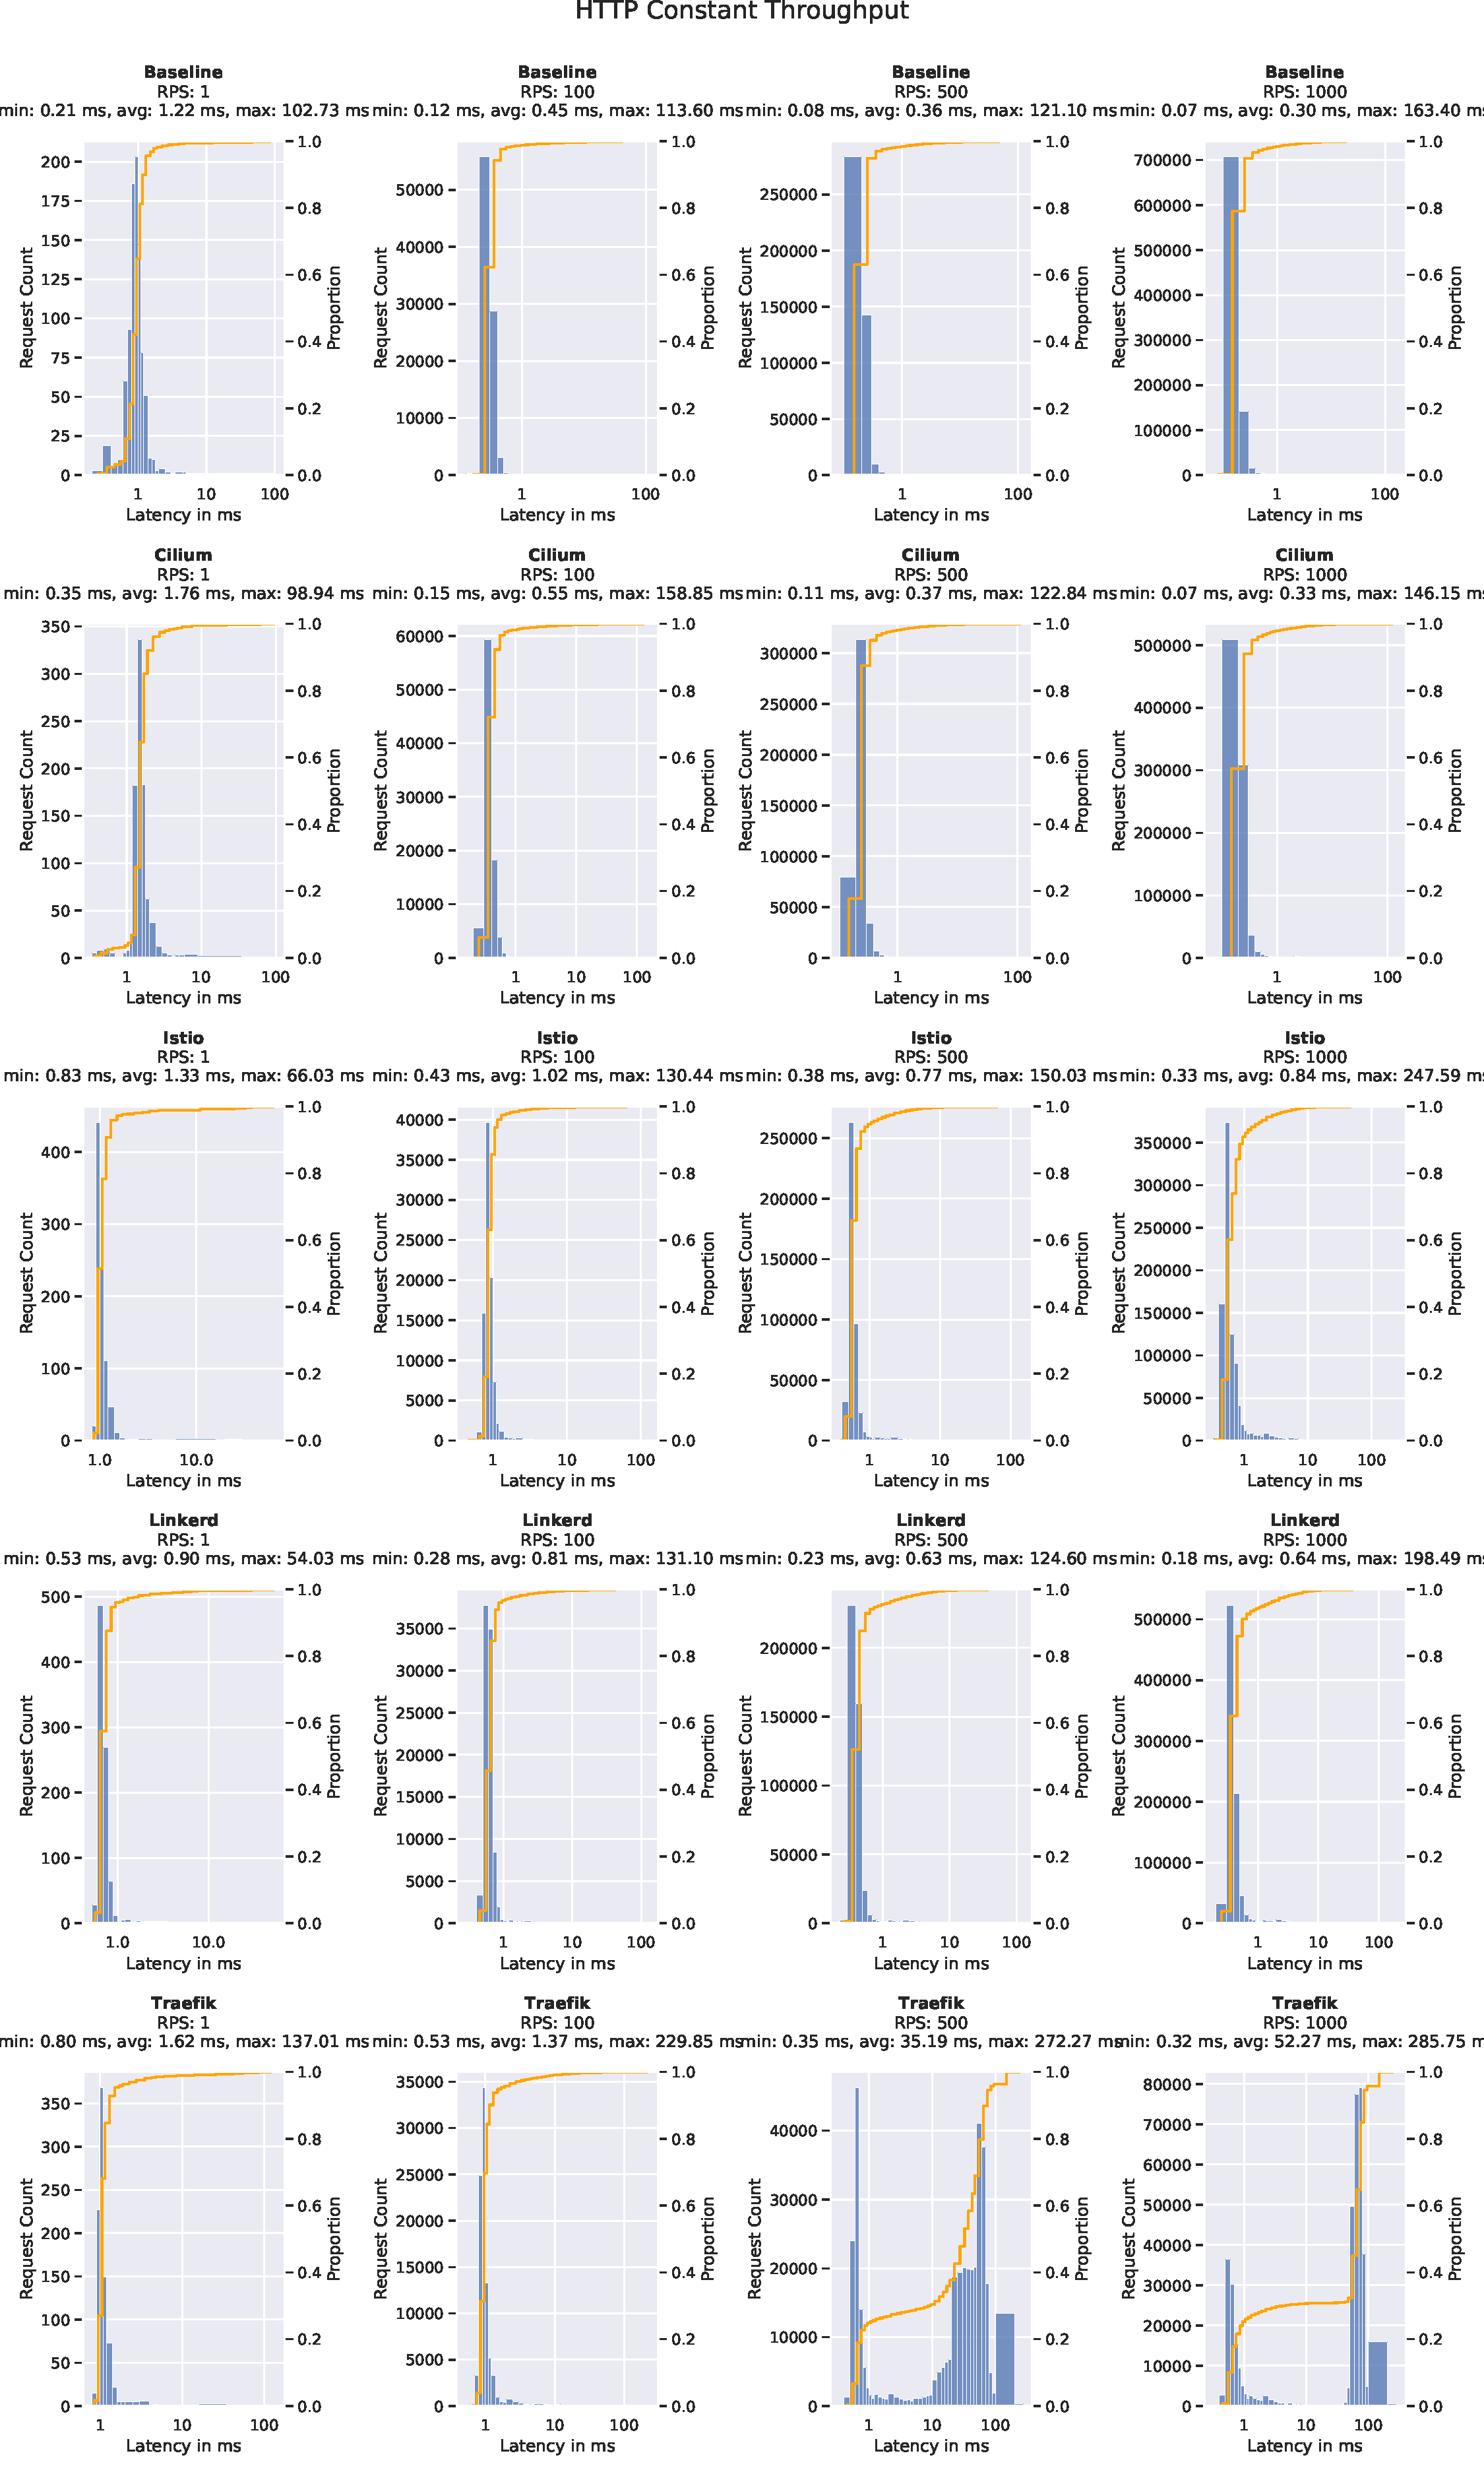
\includegraphics[width=\textwidth,height=\textheight]{5_experimental_evaluation/figures/exp_02-latency-combined-results-offset.pdf}

    \caption{\ref{exp:design:2} - Latency Results}
    
    \label{fig:exp:result:02:latency}
\end{figure}

% How to read all three figures
% - Histogram (latency)
% - Line plot (cpu/mem)
In \cref{fig:exp:result:02:latency} we present a multitude of histograms that display the request latencies measured in each experiment. Every meshed configuration is presented on a row, where each plot on that row contains the histogram for a certain level of throughput. Again, above each histogram we present descriptive statistics and also plot the cumulative density function. In \cref{fig:exp:result:02:cpu} and \cref{fig:exp:result:02:memory} we present the resource utilization metrics obtained from this experiment. Each plot in the illustrations represents a meshed configuration. The y-axis represents the system resource metric such as CPU or memory utilization. The x-axis represents the time delta since the start of the experiment. Note that the line is continuous, since all four different levels of constant throughput are measured one after another. Additionally, each line is coloured and represents a single container on the data path, i.e. target service and proxy (if applicable).

% Results:
% Distribution of traefik changed when peak is hit (~560RPS as in exp1) to bimodal
% Istio/Linkerd max suffering
% - Underlying data/bins (or log plots) show 99p 99.9p suffering
From the histograms \cref{fig:exp:result:02:latency} we can see that for most configurations the distribution stayed very similar. The most significant difference occurs at \textit{Traefik}, where the bimodal distribution occurs at a constant throughput of 500 requests per second and above. This falls in line with the observed behaviour as experienced in \ref{exp:design:1} and indicates a bottleneck of some sort. We can also observe from the descriptive statistics that the maximum values observed in these controlled environments seem to suffer for \textit{Istio}, \textit{Linkerd} and \textit{Traefik} which can be confirmed by taking a closer look at the underlying data that shows higher latency outliers in the tail ends of the spectrum in the 99th and 99.9th percentile.


\begin{figure}[h]
    \centering
    
    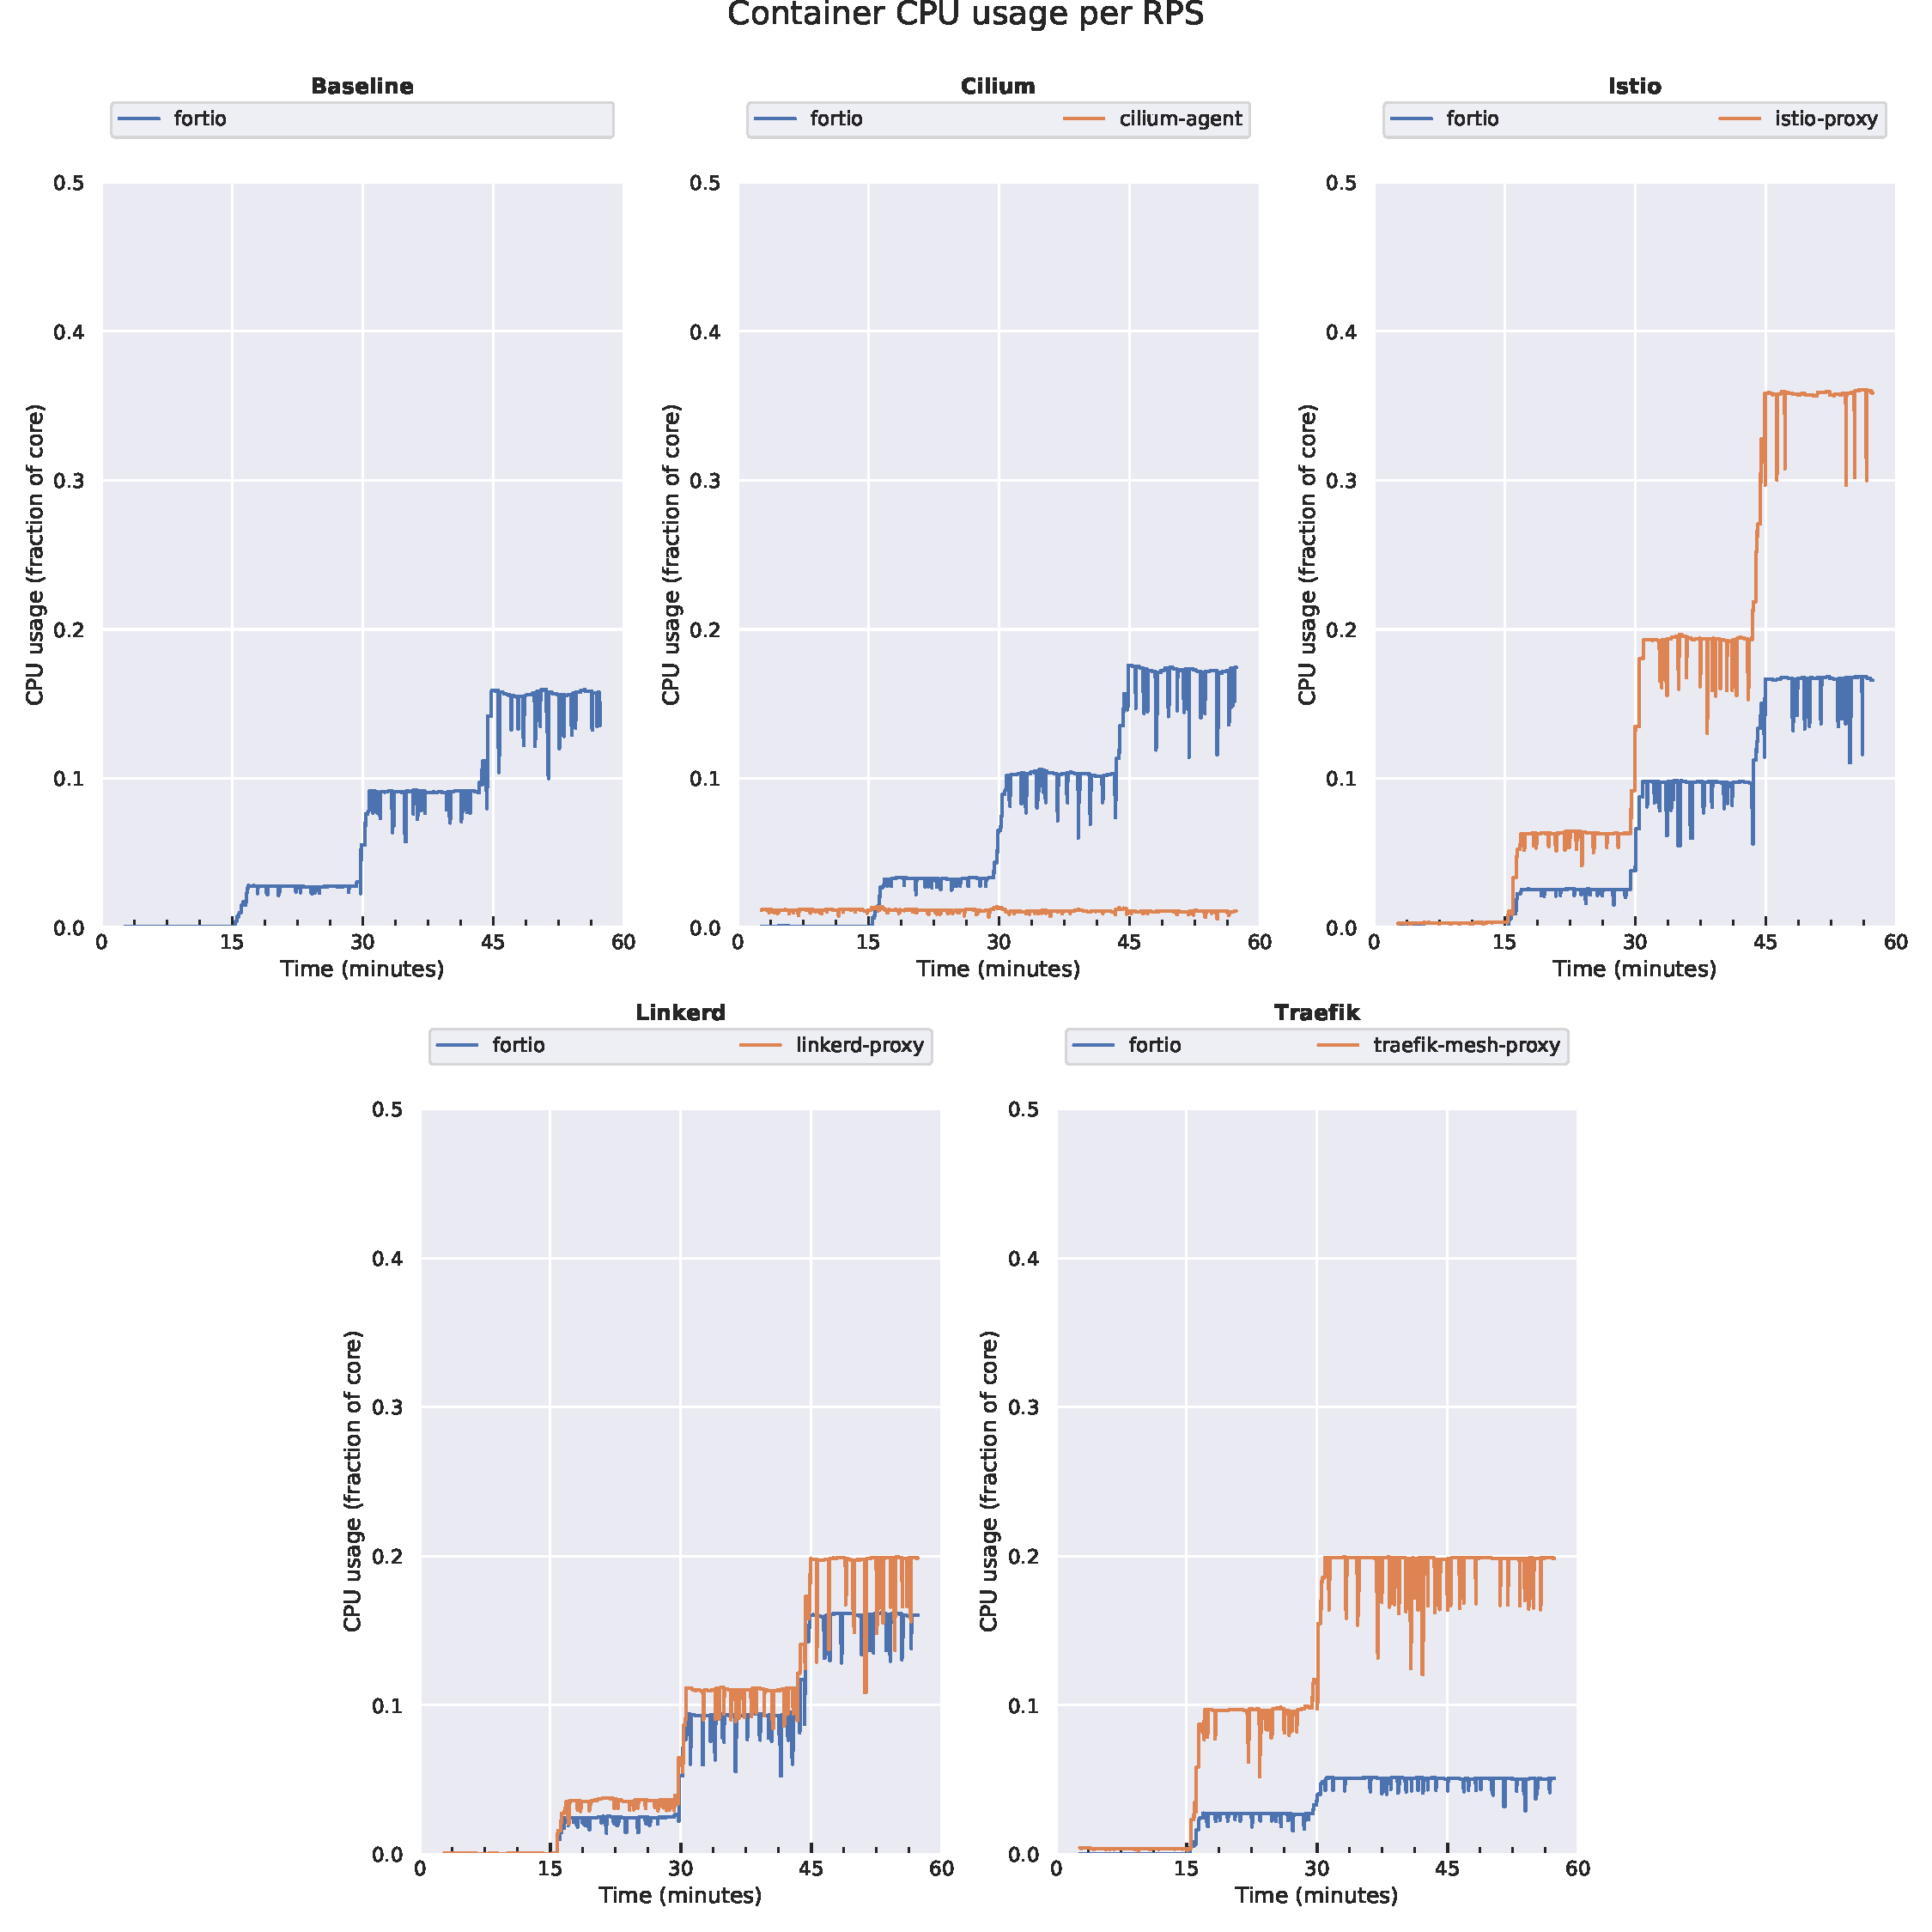
\includegraphics[width=\linewidth]{5_experimental_evaluation/figures/exp_02-cpu-results.pdf}

    \caption{\ref{exp:design:2} - CPU utilization results.}
    
    \label{fig:exp:result:02:cpu}
\end{figure}


% Linar scaling of CPU utilization service
% Istio worst scaling
% Traefik bottleneck at 500
% Memory consumtion similar at all levels
% Linkerd least amount of memory
From the CPU utilization results as depicted in \cref{fig:exp:result:02:cpu} we can observe that the increase in CPU consumption for the target service is linear to the amount of throughput applied. In the results we can observe that \textit{Cilium} seems to consume the least amount of CPU utilization and that it stays stable for each of the workloads. \textit{Istio}, on the other hand, seems to have the worst scaling regarding its CPU utilization. \textit{Linkerd} and \textit{Traefik} seem to scale similarly, however, scaling for the latter stops at the 500 RPS threshold due to its bottleneck. From the memory utilization results as depicted in \cref{fig:exp:result:02:memory} we can observe that \textit{Linkerd} consumes the least amount of memory from all meshed configurations. Another observation is that the memory footprint is similar for each of the workloads, except for the \textit{Traefik} proxy at 1 RPS, which is slightly lower. Again, all observed values are negligible for most environments.


\begin{figure}[h]
    \centering
    
    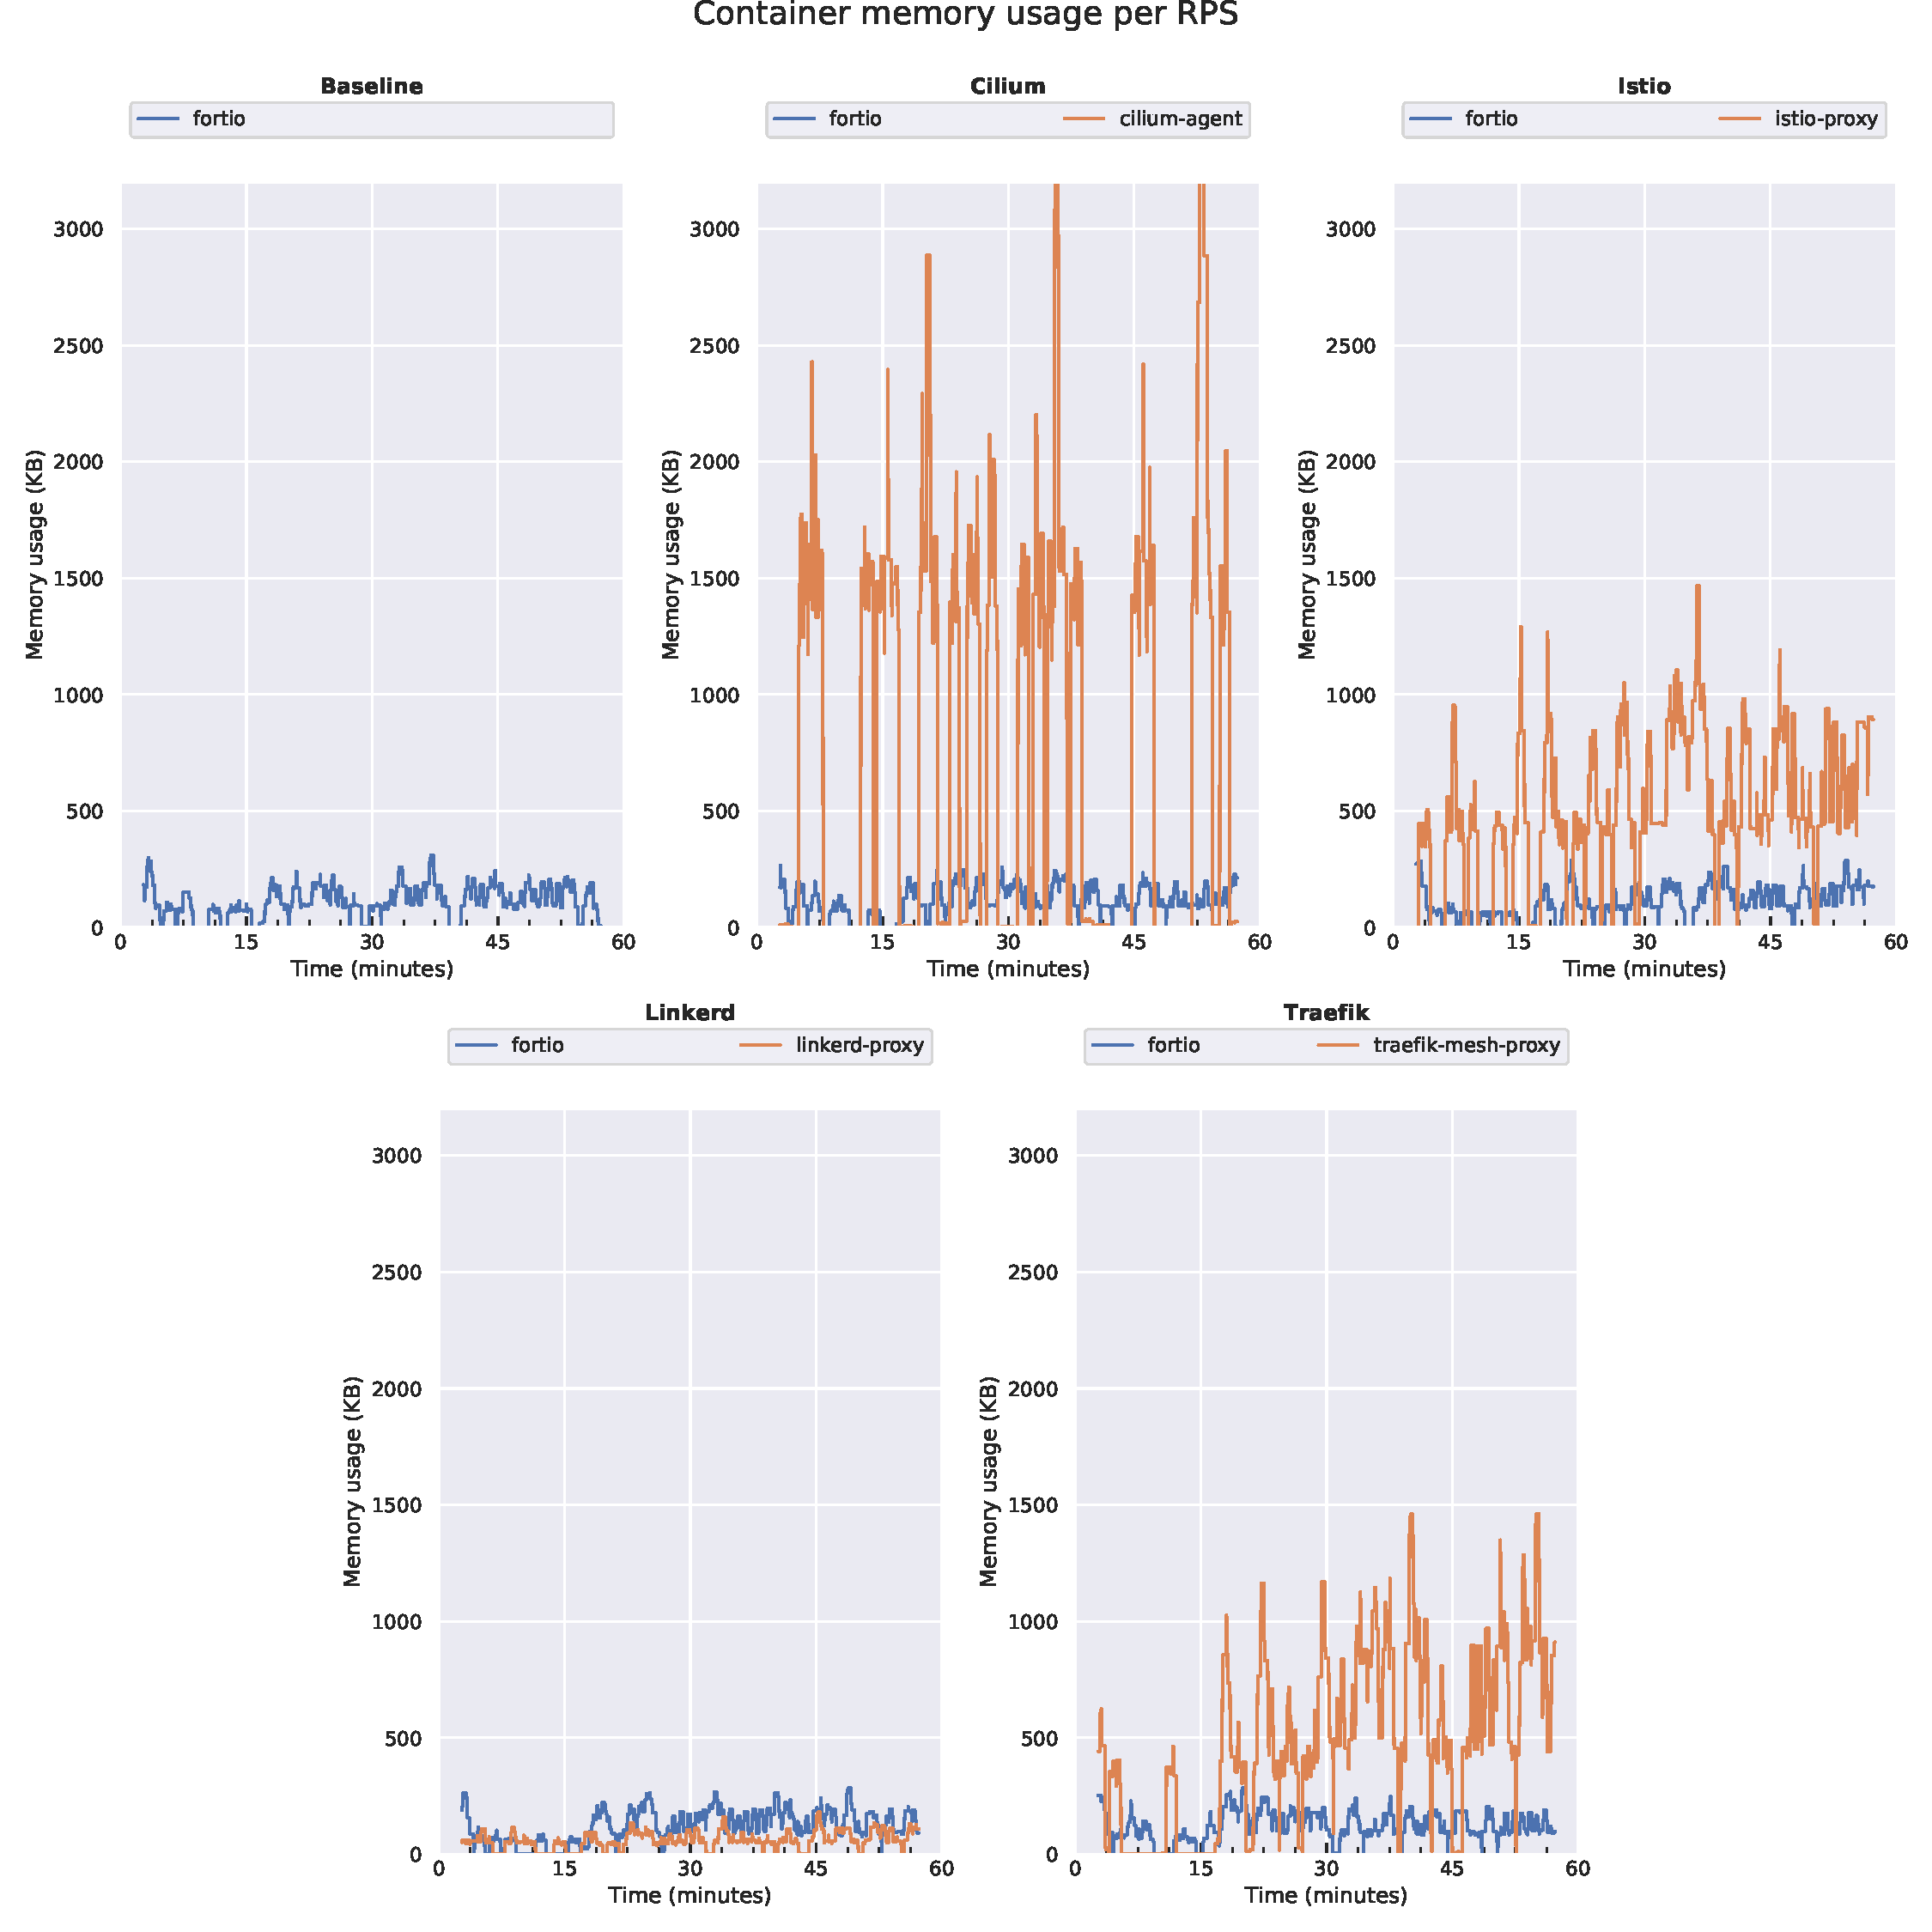
\includegraphics[width=\linewidth]{5_experimental_evaluation/figures/exp_02-mem-results.pdf}

    \caption{\ref{exp:design:2} - memory utilization results.}
    
    \label{fig:exp:result:02:memory}
\end{figure}



\subsubsection{\ref{exp:design:3} - HTTP Payload}
\label{sec:experiments:results:per-experiment:03}

In the third experiment we introduced application payloads. The goal of this experiment is to evaluate the performance of these systems with different payload sizes. The result of this experiment is depicted in \cref{fig:exp:result:03:latency}.

% Explain how to read the figure
\cref{fig:exp:result:03:latency} contains five rows of histogram results. Each of these rows contain the results of a mesh configuration and each of the columns is a result for a given payload size. The first column contains the results of a load test where the target service returns an empty response. The second and third column, however, represent the results of a load test where the target returns a payload of 1 kilobyte and 10 kilobytes respectively as indicated by the plot labels. Additional descriptive statistics are added to each plot without the throughput count as it is static at 100 requests per second for each result in the figure.


\begin{figure}[!t]
    \centering
    
    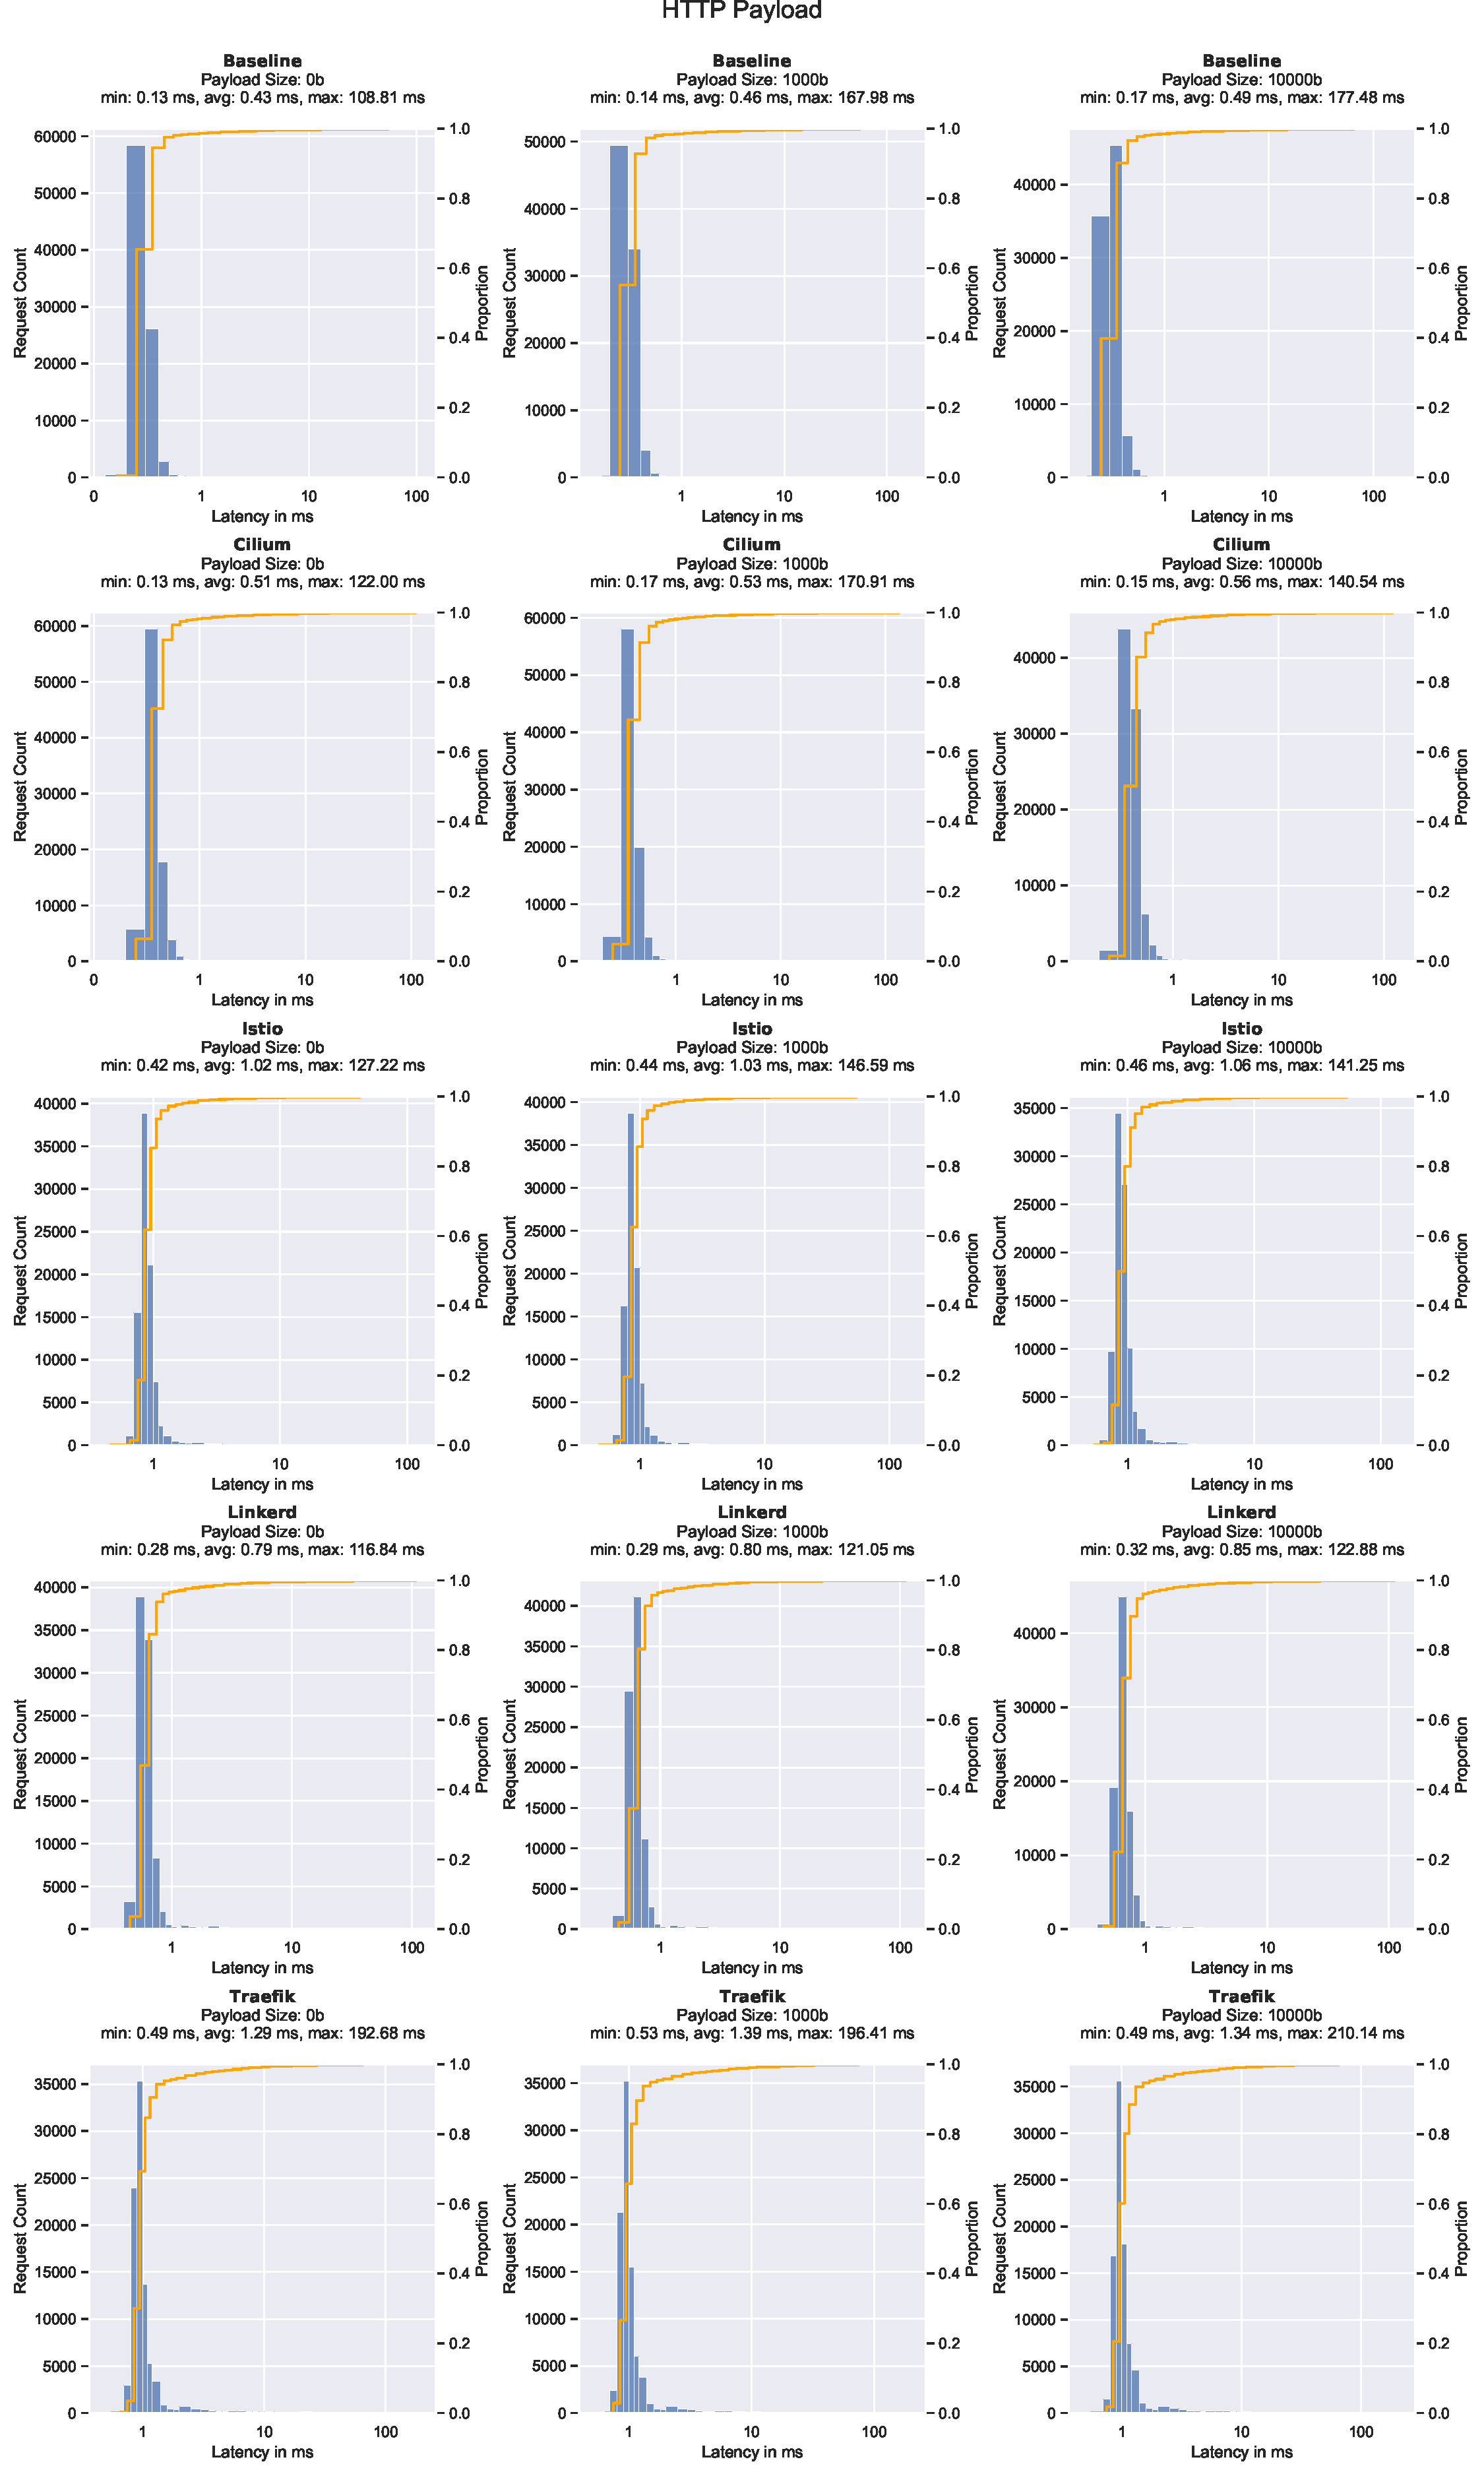
\includegraphics[width=\textwidth,height=\textheight]{5_experimental_evaluation/figures/exp_03-latency-results.pdf}

    \caption{\ref{exp:design:3} - Latency Results}
    
    \label{fig:exp:result:03:latency}
\end{figure}


% Results
% -maximum values higher
% p99.9 p99 similar
From the results of the histograms as depicted in \cref{fig:exp:result:03:latency} we can observe that the distributions remain similar for all the observed payload sizes. In fact, when inspecting the data in finer detail we observe that the tail end is nearly identical and that there is no significant difference in the tail latencies of the 99th and 99.9th percentile. 


\subsubsection{\ref{exp:design:4} - gRPC Maximum Throughput}
\label{sec:experiments:results:per-experiment:04}
% Goal: To evaluate how meshed configurations behave with alternative communication protocols.

The final experiment uses a different type of workload. In this experiment, we aim to evaluate the performance of \gls{sm} systems under alternative application level protocols. The results of this experiment can be seen in \cref{fig:exp:result:04:latency}


\begin{figure}[h]
    \centering
    
    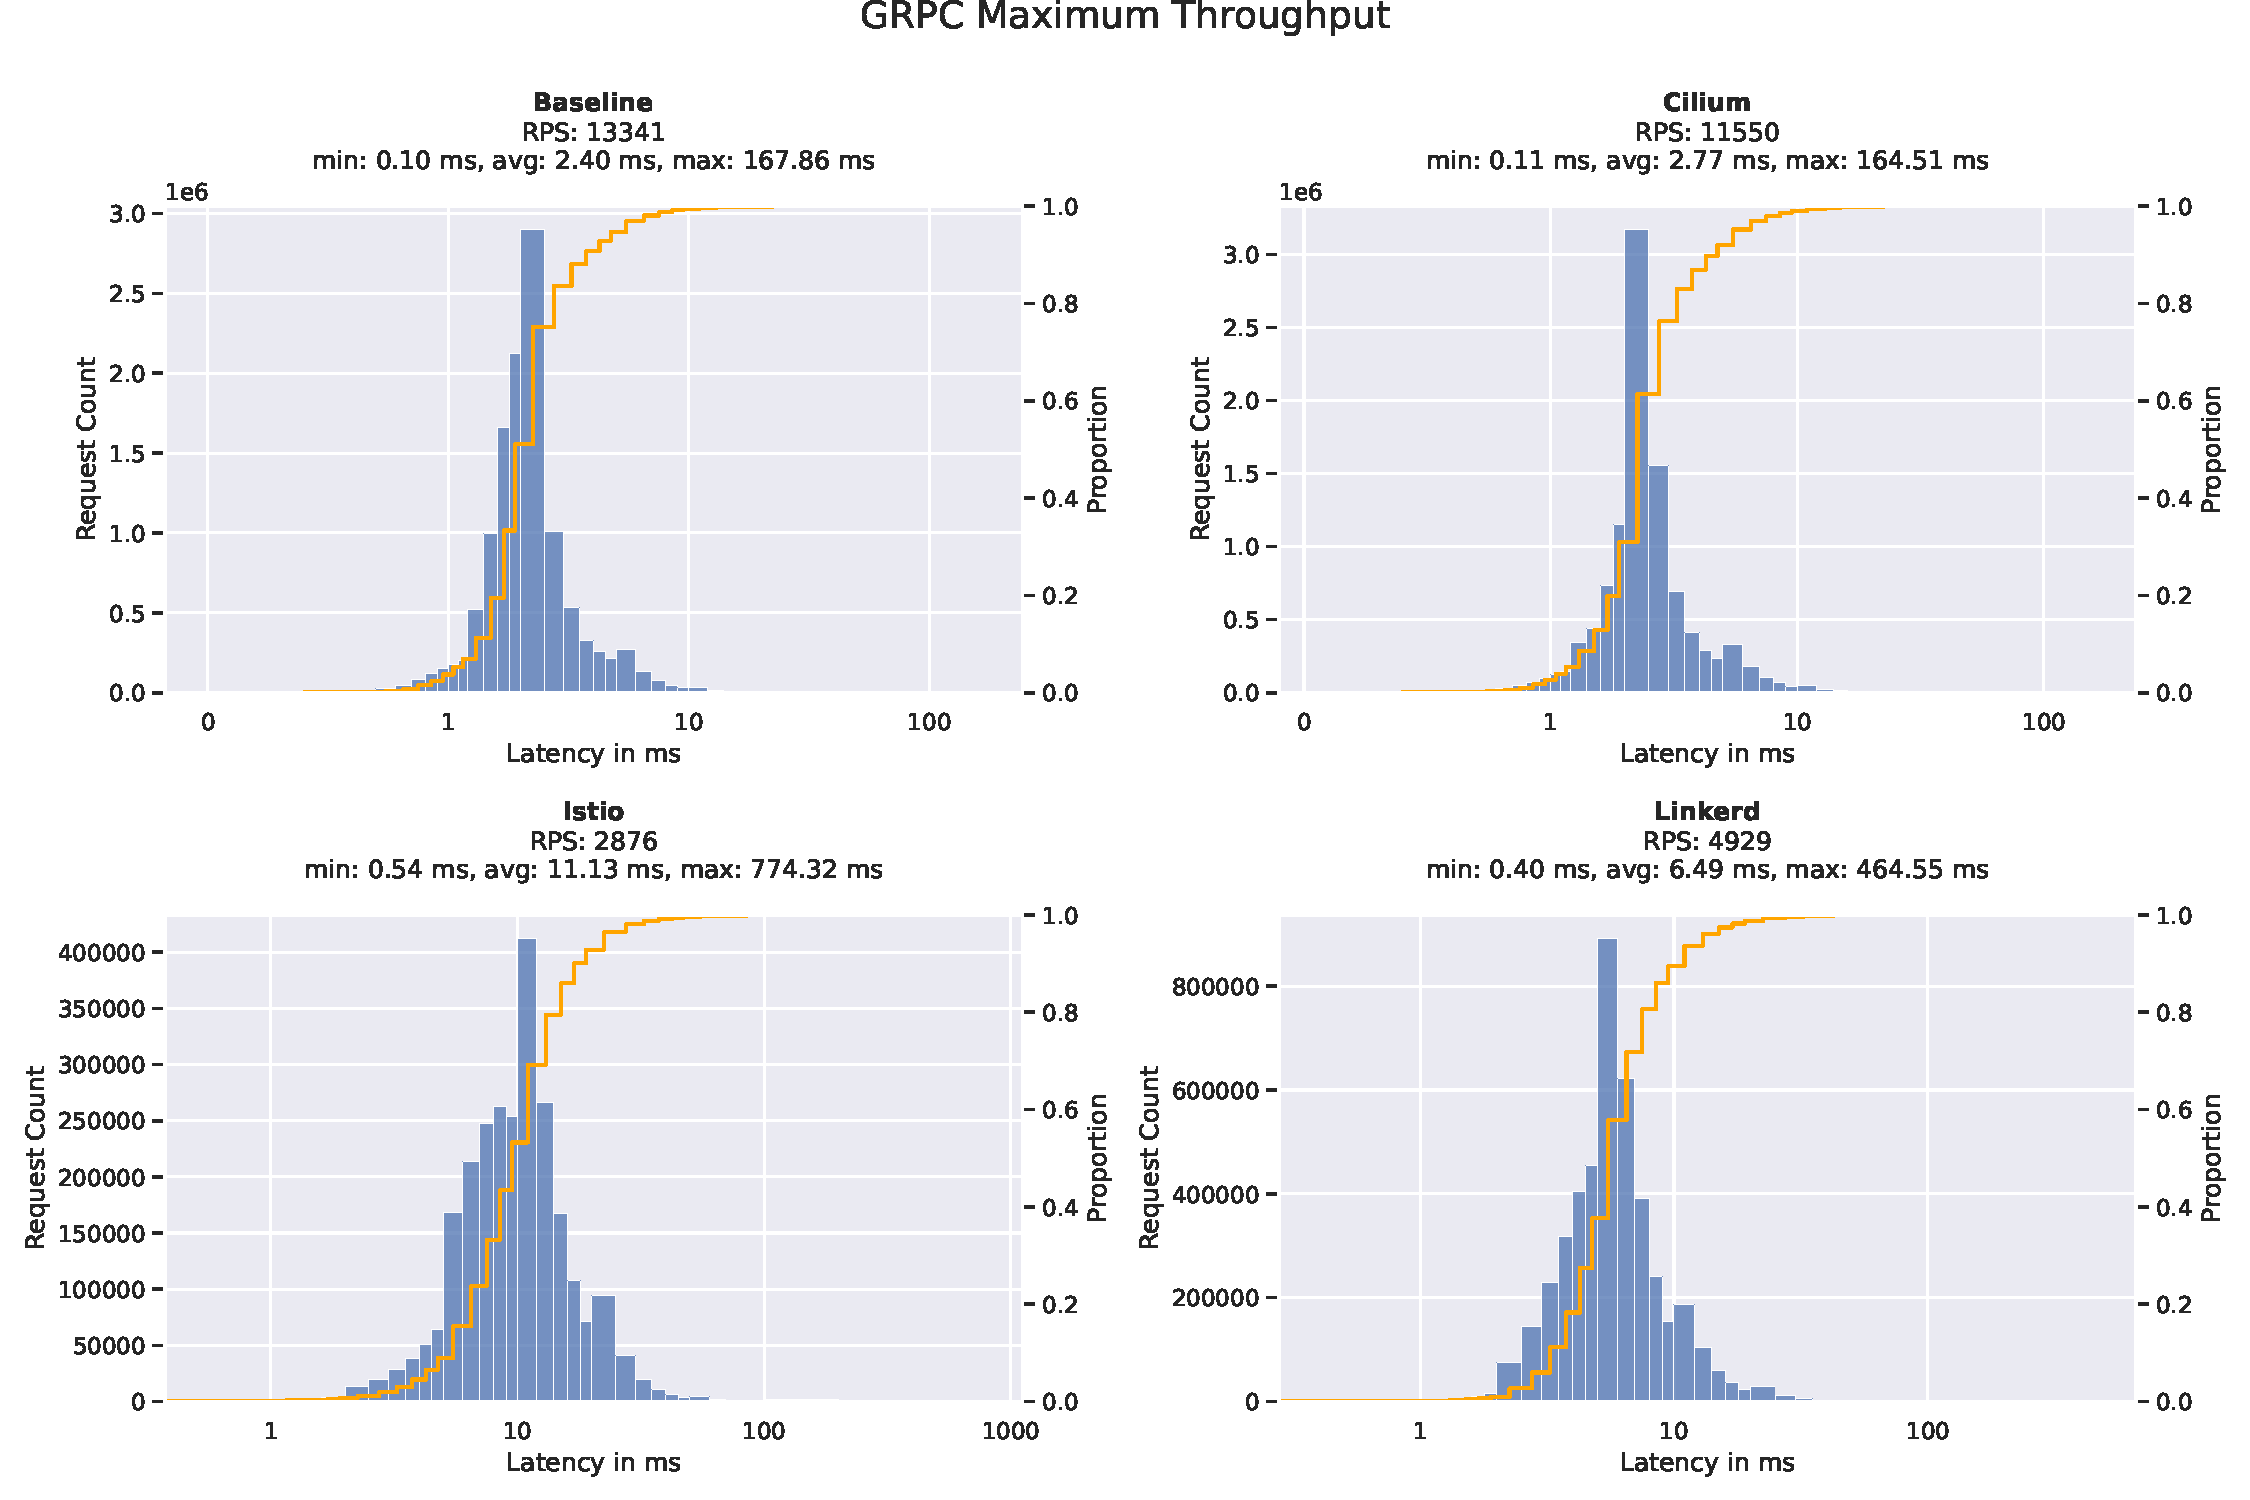
\includegraphics[width=\linewidth]{5_experimental_evaluation/figures/exp_04-latency-results.pdf}

    \caption{\ref{exp:design:4} - latency results.}
    
    \label{fig:exp:result:04:latency}
\end{figure}

% Describe plots
The histograms in \cref{fig:exp:result:04:latency} show the distribution of request latencies of the gRPC workloads for each of the mesh configurations. The y-axis on the left represents the number of requests related to the bars. The y-axis on the right indicates the proportion which is tied to the cumulative distribution function line on top of the histogram. The x-axis is once again a logarithmic axis representing the latency expressed in milliseconds. Additional descriptive metrics are presented above each plot and the actual amount of throughput reached is included as well expressed in requests per second (RPS).

% Results
% - No Traefik -> No support
% - High tail end latencies
% - Drops:
% cilium -13.424%
% istio: -78.442%
% linkerd: -63.053%

% Htpt diff
% cilium QPS diff: -16.827679769486704%
% istio QPS diff: -80.0264142981776%
% linkerd QPS diff: -54.940993873502805%
% traefik QPS diff: -97.38692130213765%
The first observation from this experiment was that the \textit{Traefik} proxy was unable to support and therefore process the gRPC requests, leading to its absence in the depicted results. Furthermore, we can see that for the meshed configurations we again see a decrease in maximum throughput achieved compared to the baseline configuration for all the meshed configurations. Similar to the HTTP experiment as discussed in \cref{sec:experiments:results:per-experiment:01}, we observe that \textit{Cilium} is performing the best out of all meshed configurations regarding its maximum throughput, losing out on $-13.42\%$ compared to the baseline. \textit{Linkerd} and \textit{Istio} have a significant drop compared to the baseline configuration, losing $-54.94\%$ and $-97.39\%$ of the maximum throughput compared to the baseline respectively. An interesting observation can be made is regarding the distributions and tail end latencies of the requests for \textit{Linkerd} and \textit{Istio}. The average requests latencies see a significant increase, with $+170.42\%$ and $+363.75\%$ compared to the baseline average respectively. This trend continues for the tail end latencies and maximum values observed as well indicating that the proxies introduce a notable performance overhead.

% istio ~38 p99
% linkerd ~22 p99